\documentclass[final]{beamer}
\mode<presentation>
  {
    \usetheme{Bright}
  }
  \usepackage{times}
  \usepackage{amsmath,amsthm, amssymb, latexsym}
  \usepackage[english]{babel}
  \usepackage[latin1]{inputenc}
  \usepackage[size=custom,width=74,height=110,scale=1.0,debug]{beamerposter} % dimension in centimeters

  %%%%%%%%%%%%%%%%%%%%%%%%%%%%%%%%%%%%%%%%%%%%%%%%%%%%%%%%%%%%%%%%%%%%%%%%%%%%%%%%%
  \graphicspath{}
  \title{Non-equilibrium Umbrella Sampling on BlueGene/P using One Sided Communication}
  \author{Alex R. Dickson$^1$, Jeff R. Hammond$^2$ and Aaron R. Dinner $^1$}
  \institute{$^1$ The University of Chicago (\texttt{adickson@uchicago.edu,dinner@uchicago.edu}) \\ $^2$ Argonne National Laboratory (\texttt{jhammond@alcf.anl.gov})}
  %%%%%%%%%%%%%%%%%%%%%%%%%%%%%%%%%%%%%%%%%%%%%%%%%%%%%%%%%%%%%%%%%%%%%%%%%%%%%%%%%
  \begin{document}
    \begin{columns}[t]
      \begin{column}{.33\linewidth}
        \begin{block}{Nonequilibrium Umbrella Sampling}
	  NEUS is an umbrella sampling algorithm that is applicable to nonequilibrium systems.  It divides the phase space of a system into different regions and conducts restricted simulations within each region.
        \end{block}
	\begin{block}{How it works}
	  The system does not obey detailed balance 
	  \begin{equation*}
	    P(\text{A})p(\text{A} \rightarrow \text{B}) \neq P(\text{B})p(\text{B} \rightarrow \text{A}) 
	  \end{equation*}
	  and does not have a known probability distribution
	  \begin{equation*}
	    P(x) \neq C\exp{-\beta V(x)}.
	  \end{equation*}

	  \textbf{The key insight:  run unbiased dynamics and restart walkers using a flux input distribution that is developed on-the-fly}

	  \vspace{20 mm}

	  \begin{columns}[t]
	    \begin{column}{.4\linewidth}
	      Each region is given a weight, that is determined using boundary crossing statistics.
	      The weights are used to build the full steady-state distribution from the regional ones.
	    \end{column}
	    \begin{column}{.25\linewidth}
	      \begin{figure}
		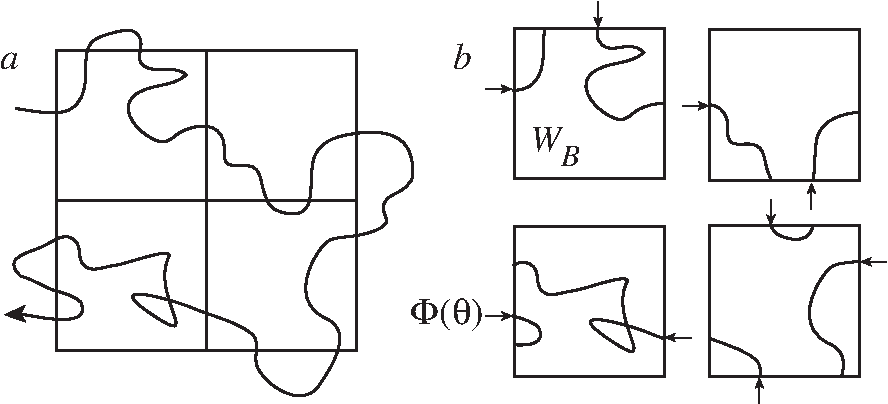
\includegraphics[width=3 in]{images/motivation2.pdf}
	      \end{figure}
	    \end{column}
	    \begin{column}{.25\linewidth}
	      \begin{figure}
		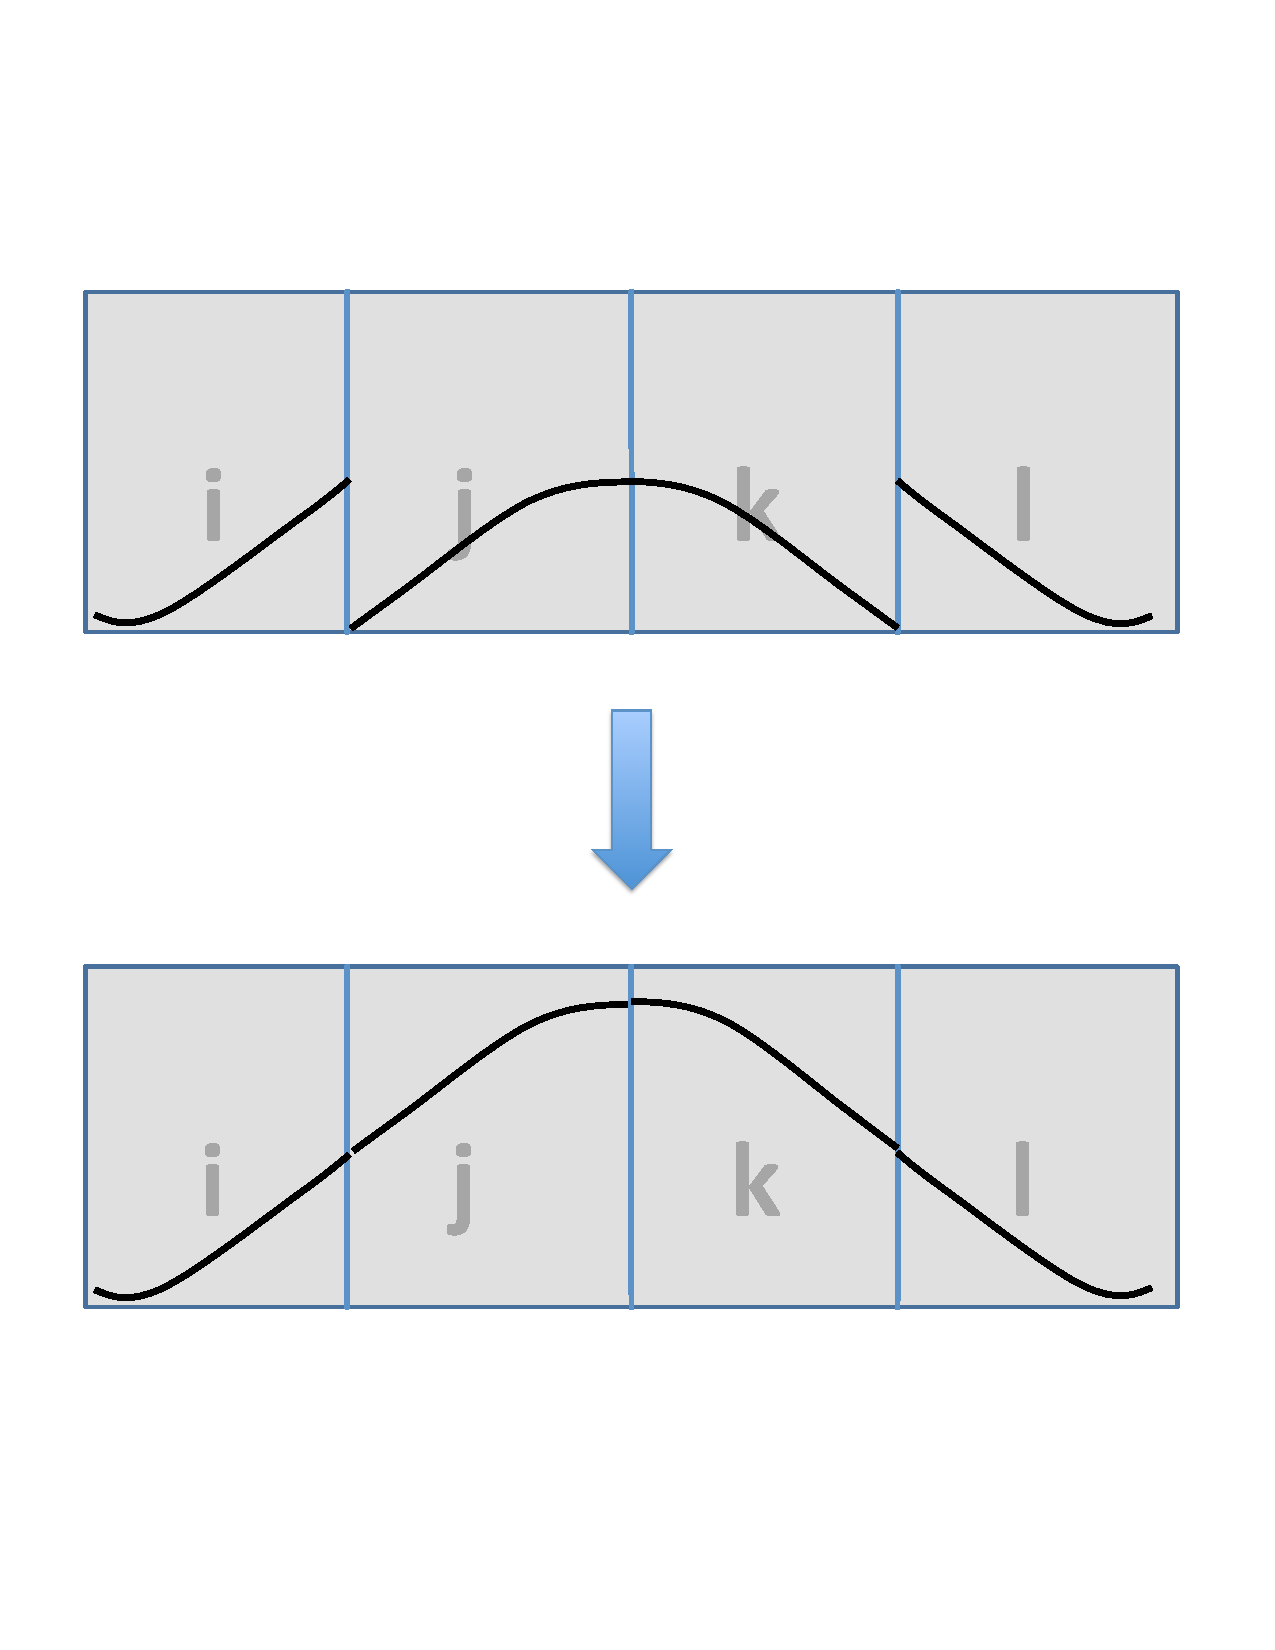
\includegraphics[width=2 in]{images/patch.pdf}
	      \end{figure}
	    \end{column}
	  \end{columns}

        \end{block}
	\begin{block}{Advanced Techniques}
	  \textbf{Strings:}

	  \begin{columns}[t]
	    \begin{column}{.65\linewidth}

	  Irregular regions can be formed by Voronoi polyhedra defined using a set of phase space points (``images'') that together form a string that winds its way from reactants to products.
	  The string is updated during sampling by periodically moving the images towards the average of the walker position in the last time interval.

	    \end{column}
	    \begin{column}{.25\linewidth}
	      \begin{figure}
		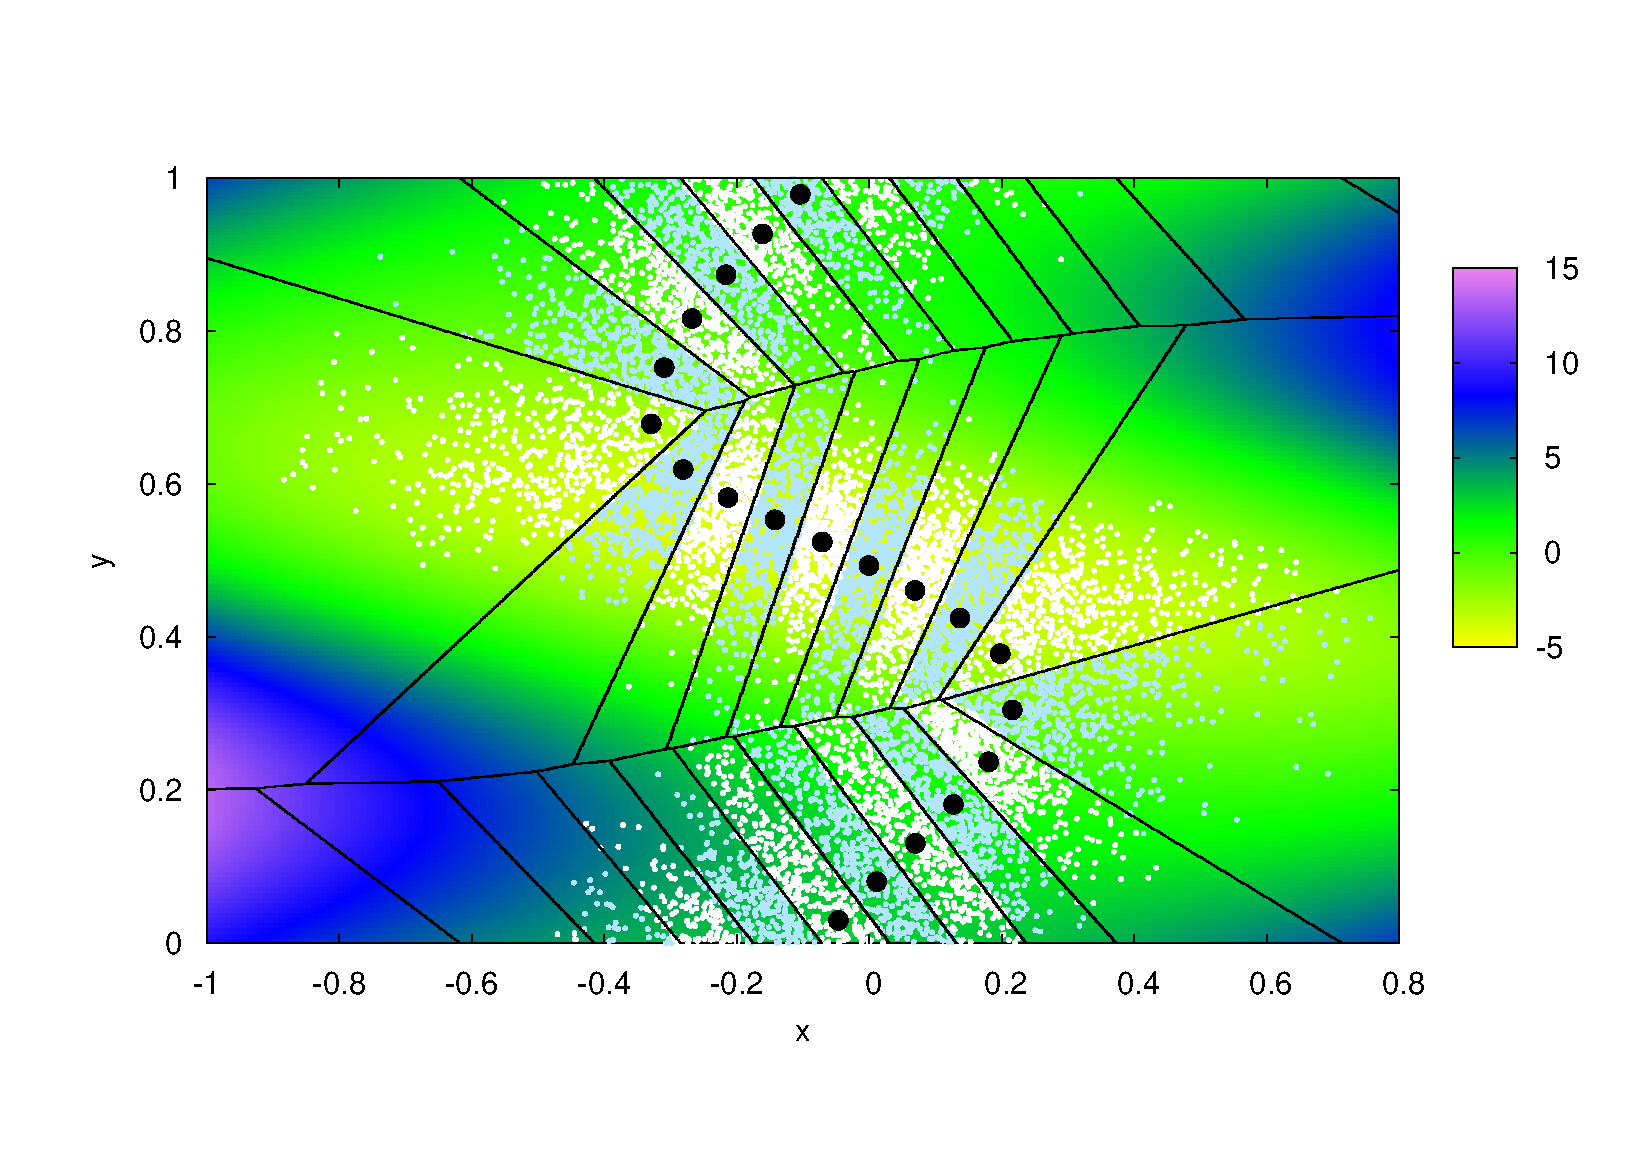
\includegraphics[width=3 in]{images/whiteandblue.pdf}
	      \end{figure}
	    \end{column}
	  \end{columns}
	  \vspace{30 mm}
	  \textbf{Separating the transition path ensemble:}

	  \begin{columns}[t]
	    \begin{column}{.65\linewidth}

	      We can also separate trajectories based on their basin of origin by defining two ensembles:  ${\cal S}_A$ for trajectories originating in basin $A$, and ${\cal S}_B$ for trajectories originating in basin $B$.
	  This allows for a better description of transition paths that are separate due to nonequilibrium path splitting, and as a bonus, it allows for the \textbf{easy calculation of transition rates!}

	  \begin{equation*}
	    \label{eq:rate}
	    k_{AB} = \frac{\overline{\Phi}_{B \mid {\cal S}_A}}{\overline{h}_A}
	  \end{equation*}

	  where $\overline{\Phi}_{B \mid {\cal S}_A}$ is the flux into basin $B$ from the ${\cal S}_A$ ensemble, and $\overline{h}_A$ is the total weight of all regions in ${\cal S}_A$.
	    \end{column}
	    \begin{column}{.25\linewidth}
	      \begin{figure}
 		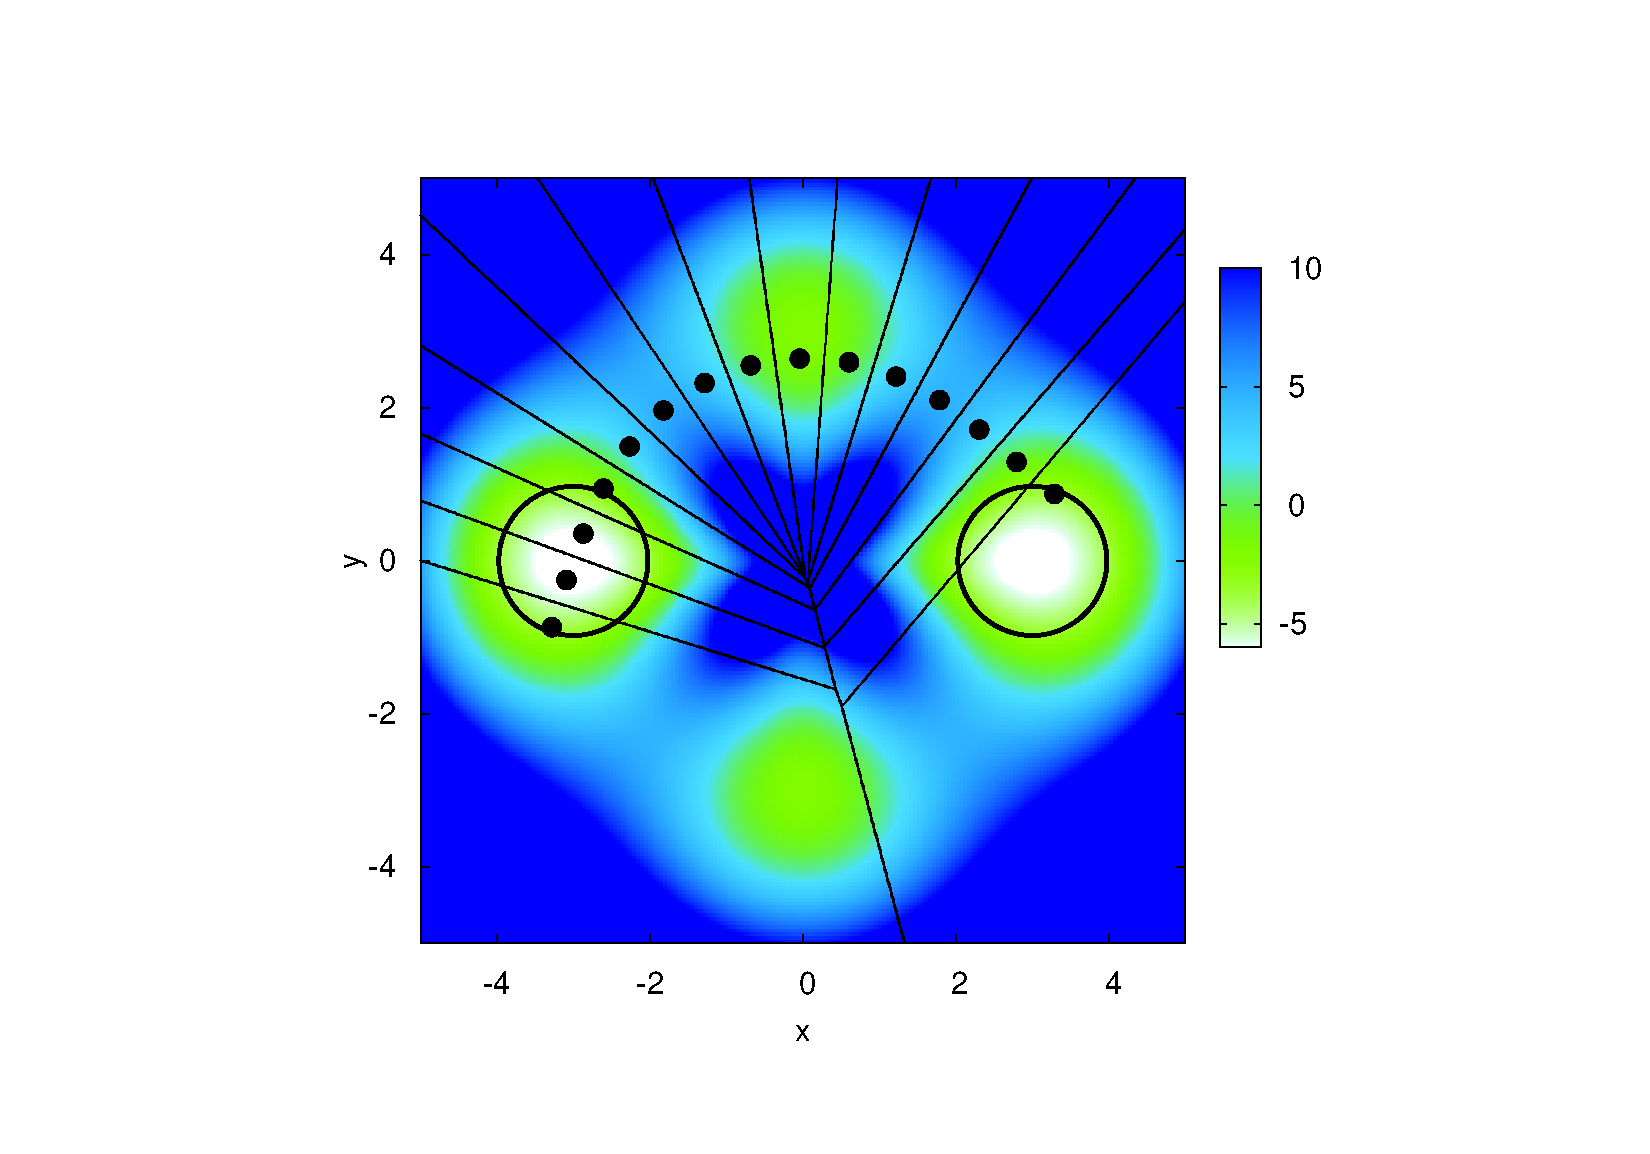
\includegraphics[width=3 in]{images/contvorf.pdf}
	      \end{figure}
	      \begin{figure}
 		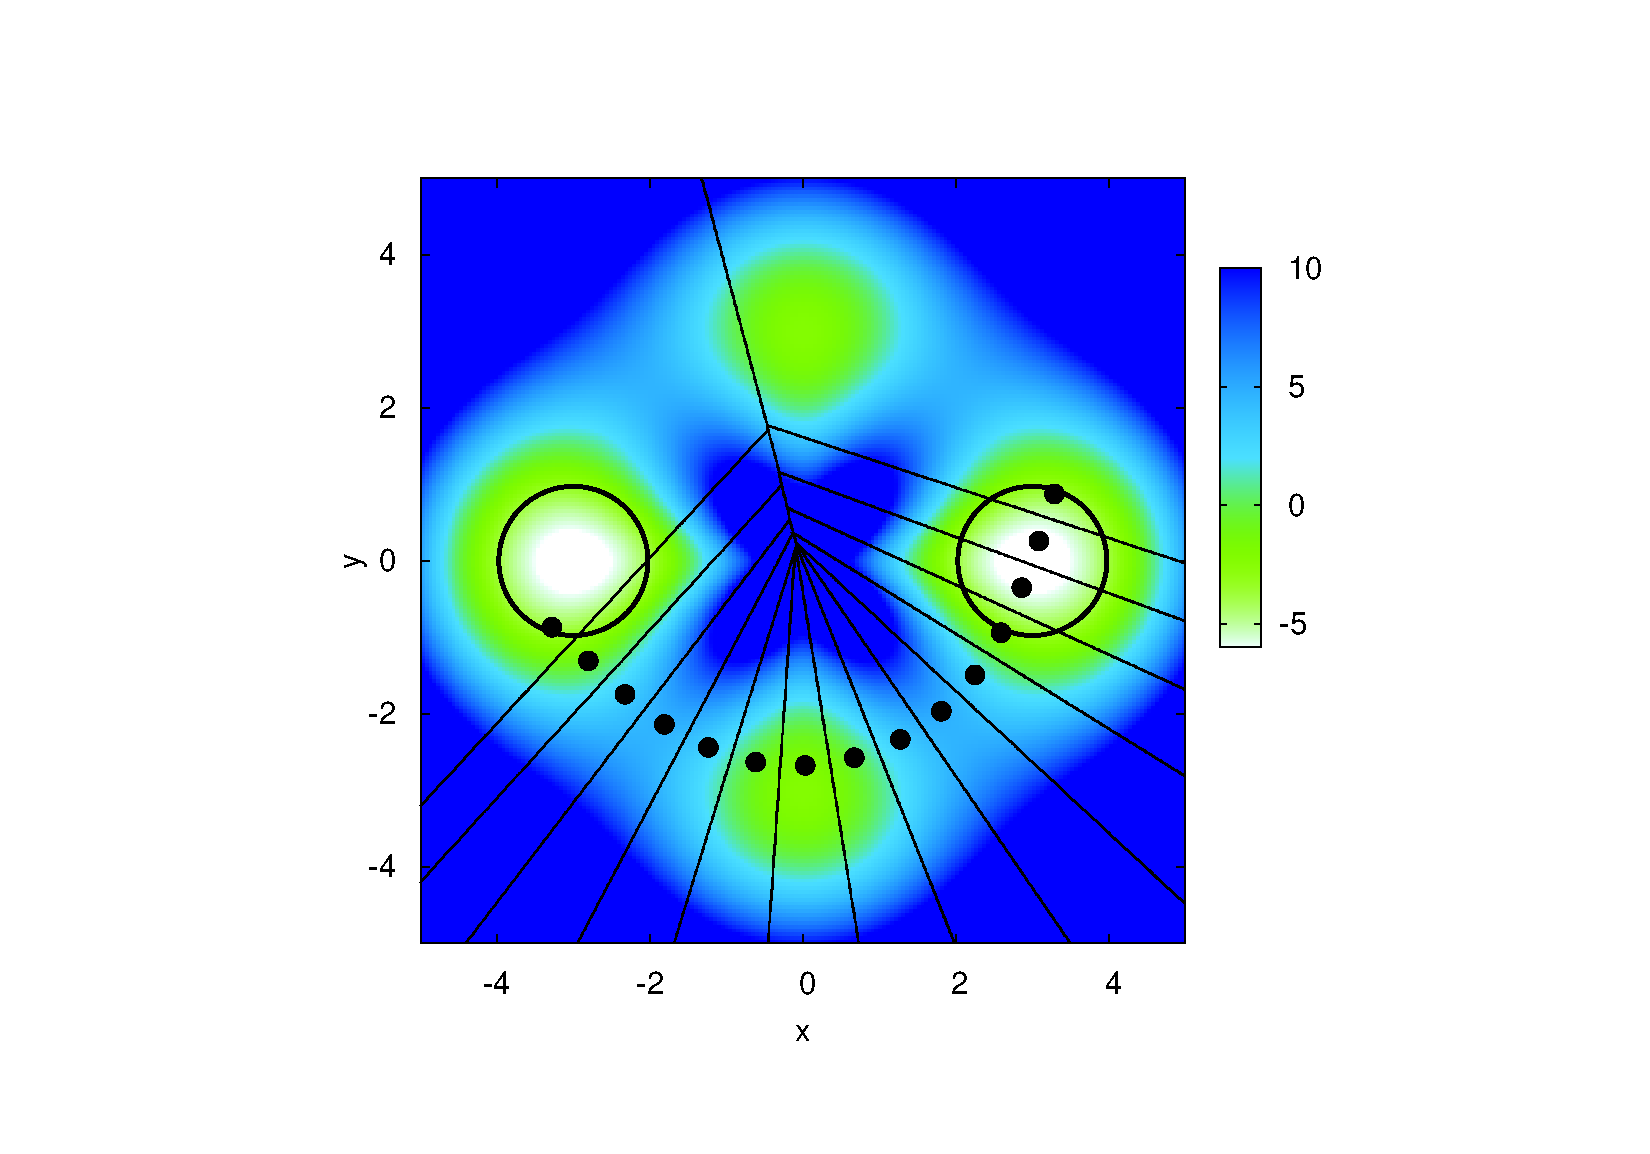
\includegraphics[width=3 in]{images/contvorr.pdf}
	      \end{figure}
	    \end{column}
	  \end{columns}
	  
        \end{block}
      \end{column}
      \begin{column}{.33\linewidth}
	\begin{block}{Examples in higher dimensions}
	  \textbf{Ising Model Under Shear}
	  \begin{columns}[t]
	    \begin{column}{.65\linewidth}
	      In the sheared Ising model, NEUS used the average magnetization of the rows as order parameters (right).  The path evolved from an arbitrary initial guess to the neighborhood of the most probable reaction path (below). 
	    \end{column}
	    \begin{column}{.25\linewidth}
	      \begin{figure}
		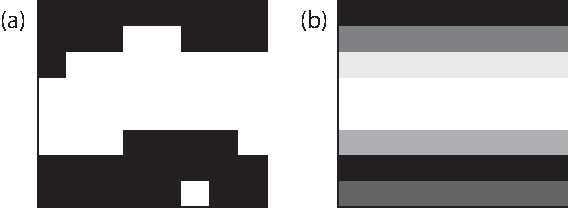
\includegraphics[width=3 in]{images/cg.pdf}
	      \end{figure}
	    \end{column}
	  \end{columns}
	  \begin{figure}
 	    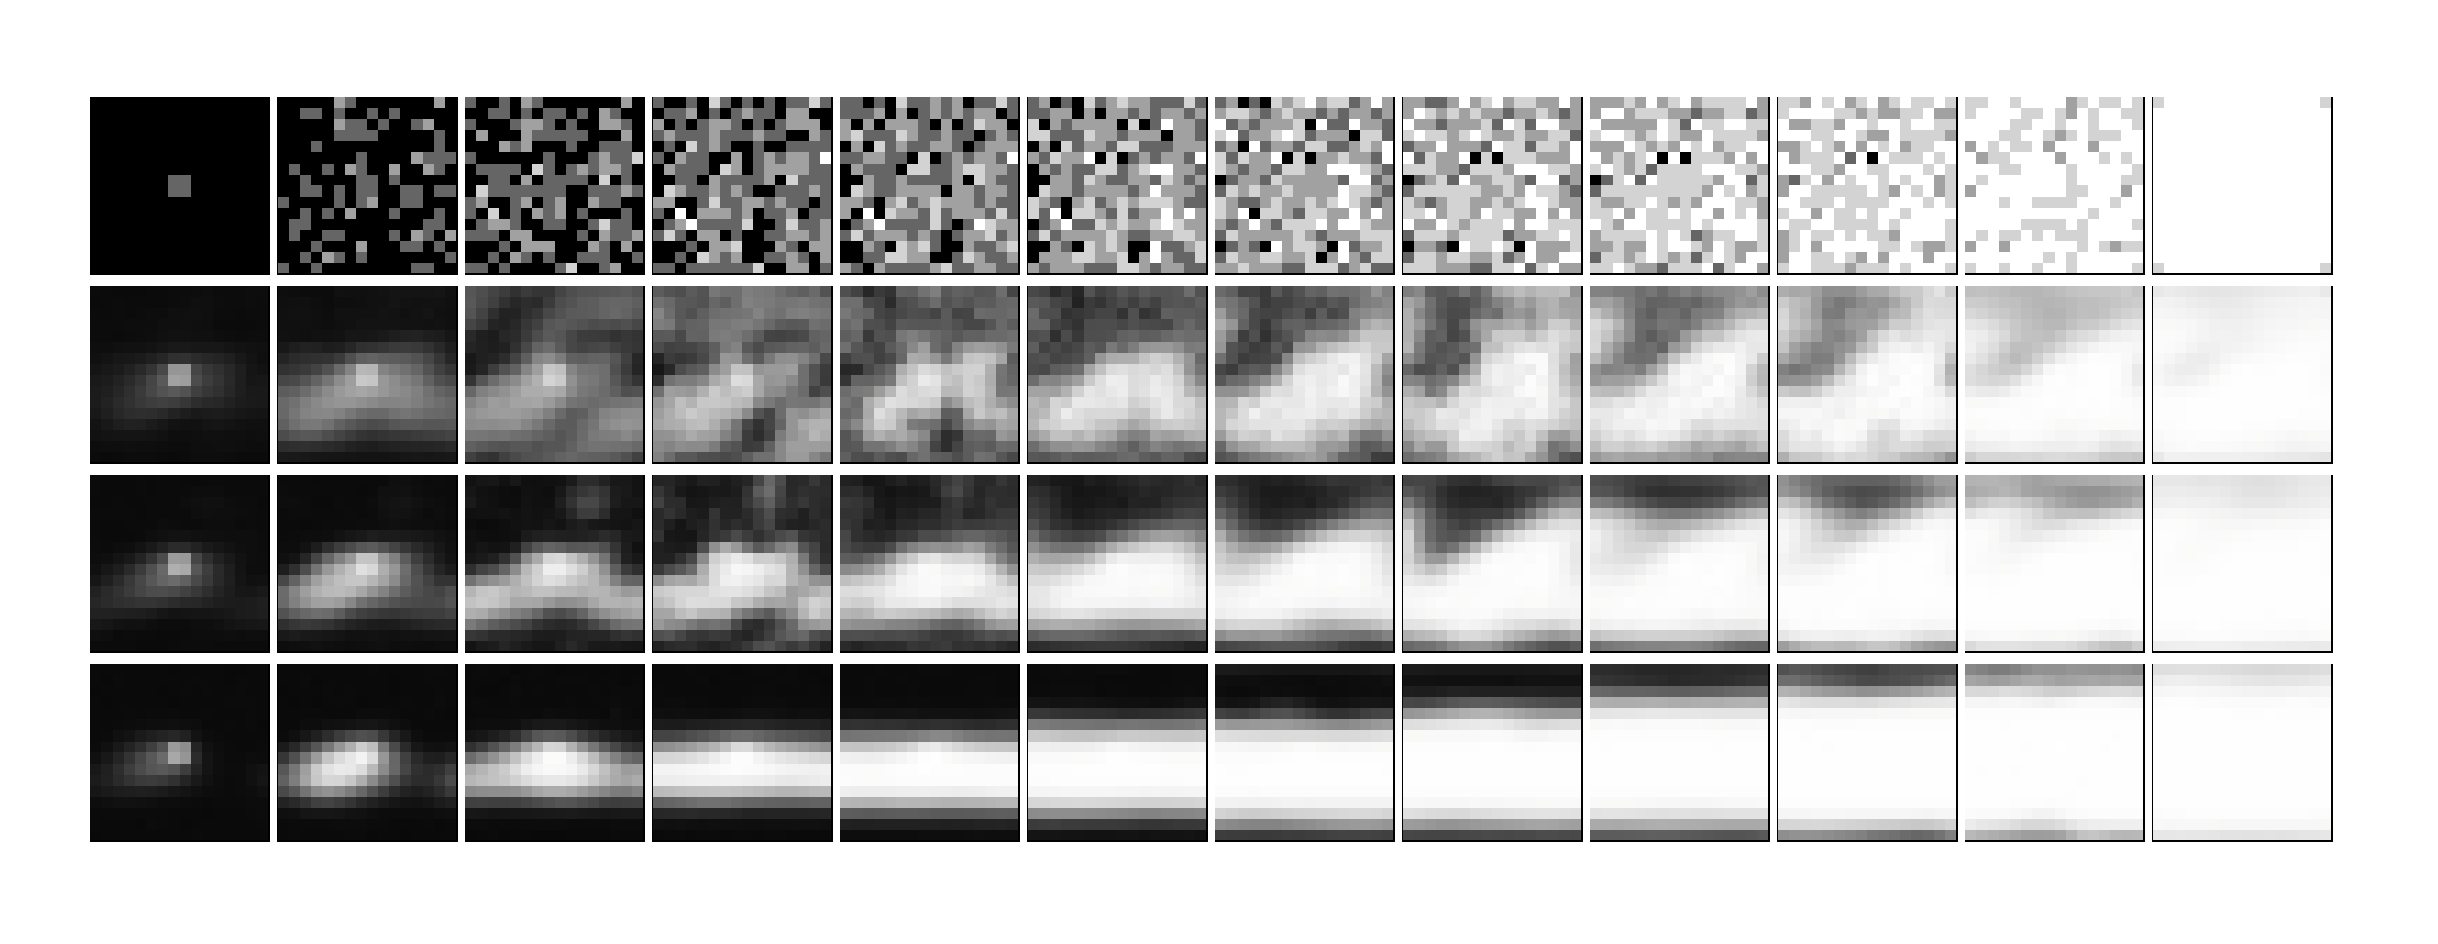
\includegraphics[width=12 in]{images/rows16.pdf}
	  \end{figure}
	  \vspace{10 mm}
	  \textbf{Circadian oscillator}

	      In a model of circadian oscillations, NEUS used the number count of each of the 22 species as order parameters.  Forward and backward path ensembles are shown below in red and blue respectively.  The algorithm was able to recover the 24h oscillatory period.
	      \begin{columns}[t]
		\begin{column}{.33\linewidth}
		  \begin{figure}
 		    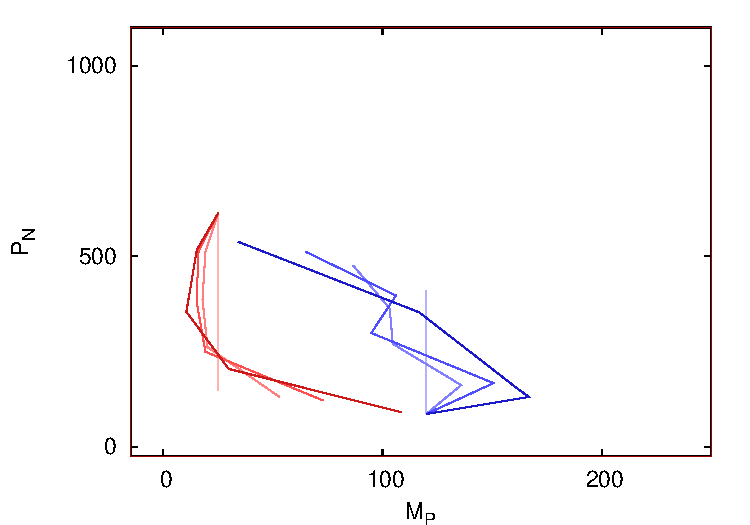
\includegraphics[width=4 in]{images/proj1umb.pdf}
		  \end{figure}
		\end{column}
		\begin{column}{.33\linewidth}
		  \begin{figure}
 		    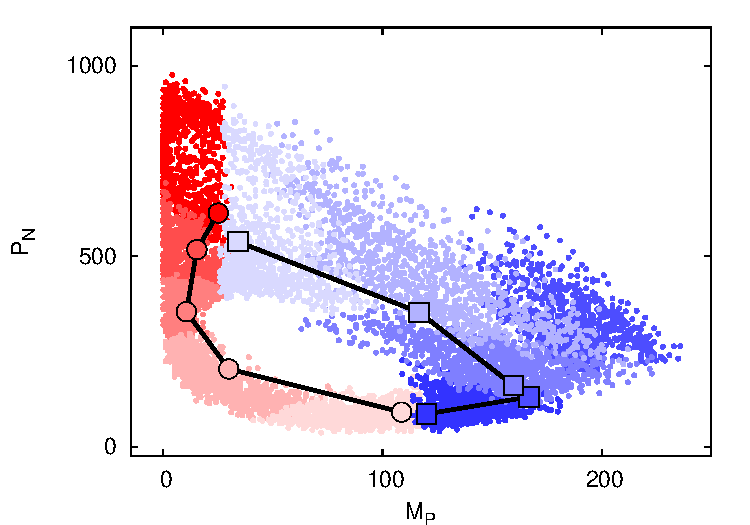
\includegraphics[width=4 in]{images/circpoints.pdf}
		  \end{figure}
		\end{column}
		\begin{column}{.33\linewidth}
		  \begin{figure}
 		    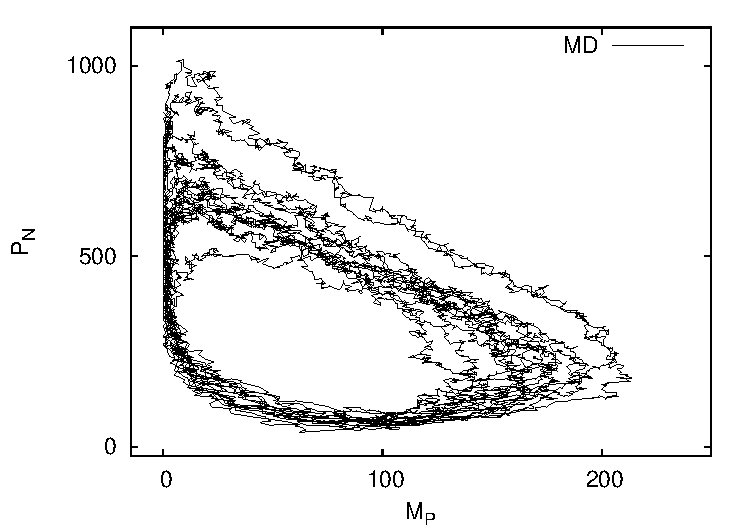
\includegraphics[width=4 in]{images/proj1md.pdf}
		  \end{figure}
		\end{column}

	  \end{columns}
        \end{block}
        \begin{block}{Parallelization using Global Arrays}
        \end{block}
      \end{column}
      \begin{column}{.33\linewidth}
        \begin{block}{Preliminary Results for a large RNA molecule under flow}
	  \textbf{The RNA Model}

	  We use a coarse-grained model where each of the 262 nucleotides is represented by a single bead.  Adjacent beads in the chain are connected with a FENE potential, and secondary and tertiary interactions are modelled with a Lennard-Jones potential.  There are also repulsive terms to keep the chain locall straight, and to mimic steric repulsion.

	  \vspace{10 mm}
	  The flow is simulated with the stochastic rotation dynamics method
	  \cite{Malevanets1999,Ihle2001,Lamura2001,Allahyarov2002}.  In that method, the
	  solvent is represented by a large number of infinitesimal particles that are 
	  grouped into cells of a lattice.  Each step of the algorithm is
	  comprised of a free streaming step and a ``collision'' step in which the velocity of each particle in the cell is rotated around the cell's average velocity vector by a random rotation matrix.
	  The RNA beads are included in the collisions, through which the solvent will influence
	  the polymer.
	  \vspace{10 mm}

	  \textbf{Evidence for long-lived stable-states}

	  The competition between the flow and the native contacts results in a rich dynamics that includes competing metastable states.
	  We are interested in the intermediate case, where contracted and extended states coexist, and transitions between them occur on long, macroscopic timescales.

	  \begin{columns}[t]
	    \begin{column}{.35\linewidth}

	      Straight-forward trajectories show evidence of these long-lived meta-stable states.  

	      (Right) shows the extension vs. time for two trajectories with different initial conditions.  
	      These trajectories were run on a single processor for 24 hours each (2 $\mu$s, with a 0.4 ps time step), and over that time did not exit their respective basins, revealing the presence of competing metastable states.
	    \end{column}
	    \begin{column}{.6\linewidth}
	      \begin{figure}
		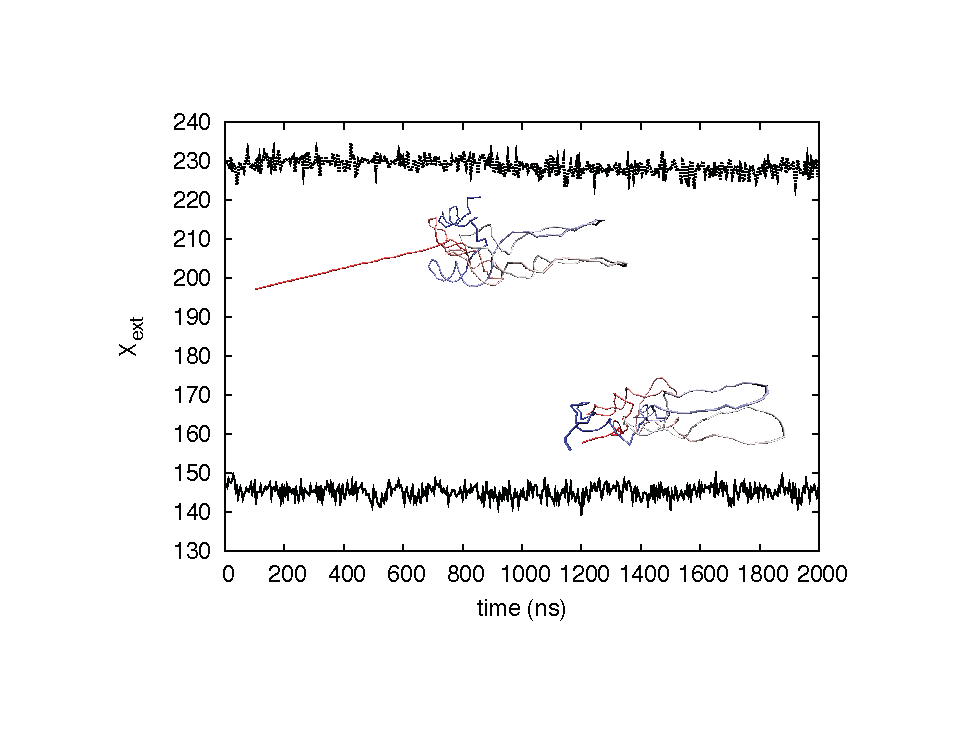
\includegraphics[width=8 in]{images/ext_fig.pdf}
	      \end{figure}
	    \end{column}

	  \end{columns}	  

	  \textbf{Scaling}

	  In preliminary measurements, we are able to acheive strong scaling to 8192 processors (2048 nodes on BlueGene/P) with 96\% efficiency.

	  \begin{figure}
	    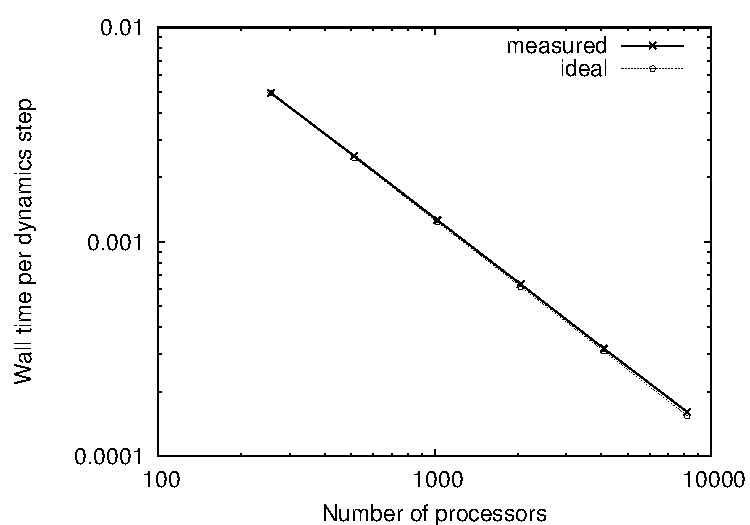
\includegraphics[width=6 in]{images/scale.pdf}
	  \end{figure}

        \end{block}
      \end{column}
    \end{columns}
  \end{document}